\documentclass[12pt, a4paper]{report}
\usepackage{graphicx, array, amsthm, amssymb, amsmath, algorithm, algpseudocode, float, xcolor, thmtools, thmbox}
\usepackage[english]{babel}

\makeatletter
\renewcommand\thmbox@headstyle[2]{\bfseries #1}
\makeatother
\newtheorem[style=M,bodystyle=\normalfont]{theorem}{Theorem}
\newtheorem[style=M,bodystyle=\normalfont]{corollary}{Corollary}
\newtheorem[style=M,bodystyle=\normalfont]{lemma}{Lemma}
\newtheorem[style=M,bodystyle=\normalfont]{definition}{Definition}


\title{Software Engineering II \\ \textit{Theory}}
\author{Christian Rossi}
\date{Academic Year 2023-2024}

\begin{document}

\maketitle

\newpage

\begin{abstract}
    The objective of the course is to teach the principals methods and processes of software engineering needed to develop complex and qualitative software.
     
    The course covers the following arguments:
    \begin{itemize}
        \item Software process and its organization.
        \item Modelling languages.
        \item Requirements analysis and definition.
        \item Software development methods and tools.
        \item Approaches for verify and validate the software.
    \end{itemize}
\end{abstract}

\newpage

\tableofcontents

\newpage

\chapter{Introduction}
    \section{Definition}
    The field of software engineering aims to find answers to the many problems that software development projects are likely
    to meet when constructing large software systems. Such systems are complex because of their sheer size, because they are 
    developed by a team involving people from different disciplines, and because they will be modified regularly to meet 
    changing requirements, both during development and after installation. 
    \begin{definition}
        \emph{Software engineering} is a methodological and managerial discipline concerning the systematic production and 
        maintenance of software products that are developed and maintained within anticipated and controlled time and cost limits.
    \end{definition}
    
    The programmer develops a complete software and works on known specifications individually. Instead, the software engineer 
    identifies requirements and develop specifications, designs components that will be combined with others and works in a team.
    The main skills of a software engineer are: technical, managerial, cognitive, organizational.

    \section{History}
    Initially, the software was considered as an art. The computers were used for computing to solve mathematical problems and 
    the designers were also the users. The first programs were created with low-level languages and had high resources constraints. 
    
    When the request for new custom software exploded the art became a craft: the developer started to create programs also 
    for the people with new high-level languages. At the end of this period there were a "software crisis" due to increasing software 
    complexity and lack of effective software development techniques. 
    
    To solve this problem in 1968 was defined the term \emph{software engineering} in a NATO conference. 
    The main focuses of this conference was on: 
    \begin{itemize}
        \item Development of software and standards.
        \item Planning and management.
        \item Automation.
        \item Modularization.
        \item Quality verification.
    \end{itemize}

    \section{The process and product}
    The developing of a software program needs a process. Both software and processes have a quality and the software engineer 
    needs to reach the optimal quality because the process modifies the final output.
    
    The software is different from traditional types of products because it is: 
    \begin{enumerate}
        \item Intangible (difficult to describe and evaluate).
        \item Malleable.
        \item Human intensive (does not involve any trivial manufacturing process).
    \end{enumerate}
    The quality of the software is influenced by the following variables: development technology, process quality, people quality, 
    cost, time and schedule. The software quality attribute are:
    \begin{itemize}
        \item Correctness: software is correct if it satisfies the specifications.
        \item Reliability: probability of absence of failures for a certain time period.
        \item Robustness: software behaves reasonably even in unforeseen circumstances.
        \item Performance: efficient use of resources.
        \item Usability: expected users find the system easy to use.
        \item Maintainability.
        \item Reusability: similar to maintainability but applies to components.
        \item Portability: adaption to different target environments.
        \item Interoperability: coexist and cooperate with other applications. 
    \end{itemize}
    The process quality attribute are:
    \begin{itemize}
        \item Productivity.
        \item Unity of effort (person month).
        \item Delivered item (lines of code and function points).
        \item Timeliness: ability to respond to change requests in a timely fashion.
    \end{itemize}

    \section{Development process}
    Initially there were no reference model, so it was simple code$\&$fix. As a reaction to the software crisis mentioned before it 
    became necessary to have a model. The first complete model was the "waterfall". The key requirements of this model are:
    \begin{enumerate}
        \item Identify phases and activities.
        \item Force linear progression from a phase to the next (without returns).
        \item Standardize outputs from each phase.
        \item Software is considered like manufacturing.
    \end{enumerate}
    After this model many other flexible processes were proposed: iterative models, agile movement and DevOps.
    \begin{figure}[H]
        \centering
        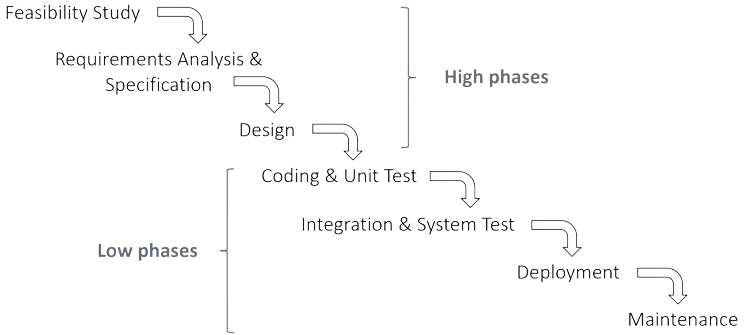
\includegraphics[width=0.75\linewidth]{images/waterfall.png}
        \caption{Waterfall process model}
    \end{figure}
    The main phases shown in the image are:
    \begin{enumerate}
        \item Feasibility study and project estimation: determines wheather the project should be started, the possible 
        alternatives and needed resources. This phase produces a \emph{Feasibility Study Document} which contains: preliminary 
        problem description, scenarios describing possible solutions, cost and schedule for the different alternatives.
        \item Requirement analysis and specification: analyze the domain in which the application takes place, identify requirements 
        and derive specification for the software. This phase produces \emph{Requirement Analysis and Specification Document}.
        \item Design: defines the software architecture (components, relation and interactions among components). The goal is to support
        concurrent development and separate responsibilities. It produces the \emph{Design Document}.
        \item Coding and unit test: each module is implemented and tested. Inspection can be used as an additional quality assurance 
        approach. Programs include their documentation. 
        \item Integration and system test: the modules are integrated into systems and integrated systems are tested. This phase 
        and the previous may be integrated in an incremental implementation scheme. 
        \item Deployment.
        \item Maintenance: the maintenance can be:
        \begin{itemize}
            \item Corrective: deals with the repair of faults or defects found.
            \item Adaptive: consist of adapting software to changes in the environment.
            \item Perfective: deals with accommodating to new or changed user requirements.
            \item Preventive: concerns activities aimed at increasing the system's maintainability. 
        \end{itemize}
    \end{enumerate}
    \begin{figure}
        \centering
        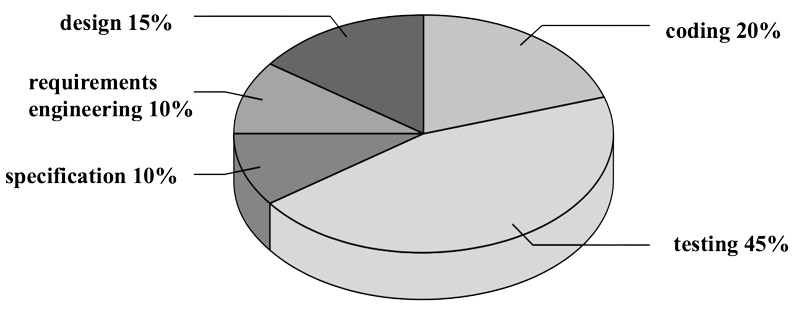
\includegraphics[width=1\linewidth]{images/effort.png}
        \caption{Effort in each phase}
    \end{figure}
    The principal problems with software evolution are:
    \begin{itemize}
        \item It is almost never anticipated and planned.
        \item Software is very easy to change (changes applied directly to the code that causes inconsistent state of project documents).
    \end{itemize}
    To face properly the evolution we need a good engineering practice that consist in two main steps: modify the design and then change 
    the implementation and apply changes consistently in all documents. In fact, one of the main goal of software engineering is to create 
    software that must be designed to accommodate future changes reliably and cheaply. 
    
    Waterfall model is a black-box system because the company that requests the software makes requirements and doesn't interact during 
    the development phase. If we need more transparency with the customer we need to use a different development model (that allows the 
    customer to give feedback regularly). With every interaction with the customer is possible to check two main things:
    \begin{itemize}
        \item Validation: check if the product follows the customer's requests.
        \item Verification: check if the product works in the right way.
    \end{itemize}
    
    The idea of flexible process is to adapt to changes, in particular the requirements and specification. The idea is to have incremental 
    processes and be able to get feedback on increments. They exists in many forms, for example: SCRUM, extreme programming, incremental 
    releases and rapid prototyping, DevOps, $\dots$
    
\newpage

\chapter{Requirements engineering}
    \section{Definition}
    The primary measure of success of a software system is the degree to which it meets the purpose for which it was intended.
    \begin{definition}
        Software systems \emph{requirements engineering} is the process of discovering that purpose, by identifying stakeholders and their needs, and documenting these in a form that 
        is amenable to analysis, communication, and subsequent implementation. 
    \end{definition}
    The important issues of this phase are: identify stakeholders, identify their needs, produce documentation and analyse, communicate and implement requirements. Another possible 
    definition is the following. 
    \begin{definition}
        \emph{Requirements engineering} is the branch of software engineering concerned with the real-world goals for, function of, and constraints on software systems. It is also 
        concerned with the relationship of these factors to precise specifications of software engineering behaviour, and to their evolution over time and across software families. 
    \end{definition}

    \section{Importance and difficulties}
    The requirements given from the customer can be classified in three main types:
    \begin{itemize}
        \item Functional: describes the interaction between the system and its environment independent from implementation. They are the main goals that the software has to fulfill.
        \item Nonfunctional: user visible aspects of the system not directly related to functional behaviour.
        \item Constraints: imposed by the client or the environment in which the system operates.
    \end{itemize}
    The nonfunctional requirements are constraints on how functionality has to be provided to the end user. They are independent of application domain but the application domain 
    determines: their relevance and their prioritization. They are also called Quality of Service attribute. 
    \begin{figure}[H]
        \centering
        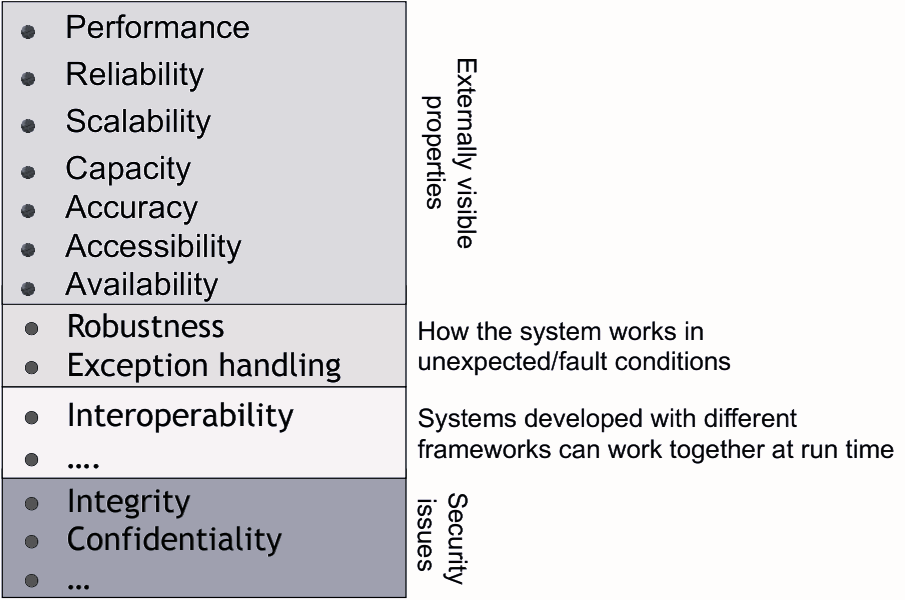
\includegraphics[width=0.75\linewidth]{images/QoS.png}
        \caption{Some relevant QoS characteristics}
    \end{figure}

    \section{Requirement engineering process}
    Poor requirements are ubiquitous. Requirement engineering is also hard and critical because a problem with the initial phases can be up to two hundred times costly in the final 
    phase. 
    \begin{figure}[H]
        \centering
        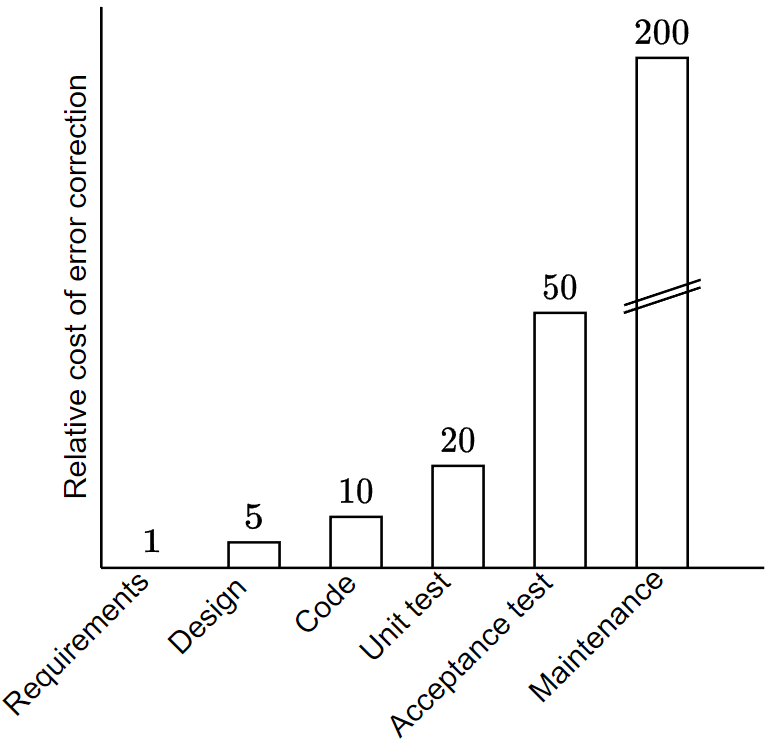
\includegraphics[width=0.75\linewidth]{images/requirements.png}
        \caption{Cost of late correction [Boehm, 1981]}
    \end{figure}
    Requirement engineering is so complex because of: composite systems. more than one system, multiple abstraction levels, multiple concerns and multiple stakeholders with different
    background.
    
    The requirement engineers needs to: 
    \begin{itemize}
        \item Eliciting information (project objectives, context and scope; domain scope and requirements).
        \item Modelling and analysis (goals, objects, use cases and scenarios).
        \item Communicating requirements (analysis feedback, RASD document, system prototypes).
        \item Negotiating and agreeing requirements (handling conflicts and risks; helping in requirement selection and prioritization).
        \item Managing and evolving requirements (managing requirements during development: backward and forward traceability; managing requirements changes and their impacts).
    \end{itemize}

    \section{World-machine relationship}
    The machine indicates the portion of system to be developed, while world indicates the portion of the real-world affected by the machine. The purpose of the machine is always in 
    the world. 
    
    Requirements engineering is concerned with phenomena occurring in the world as opposed to phenomena occurring inside the machine. We can say that requirements models are models 
    of the world. 
     
    Some world phenomena are shared with the machine. This type of phenomena can be: 
    \begin{itemize}
        \item Controlled by the world and observed by the machine.
        \item Controlled by the machine and observed by the world.
    \end{itemize}
    \begin{figure}[H]
        \centering
        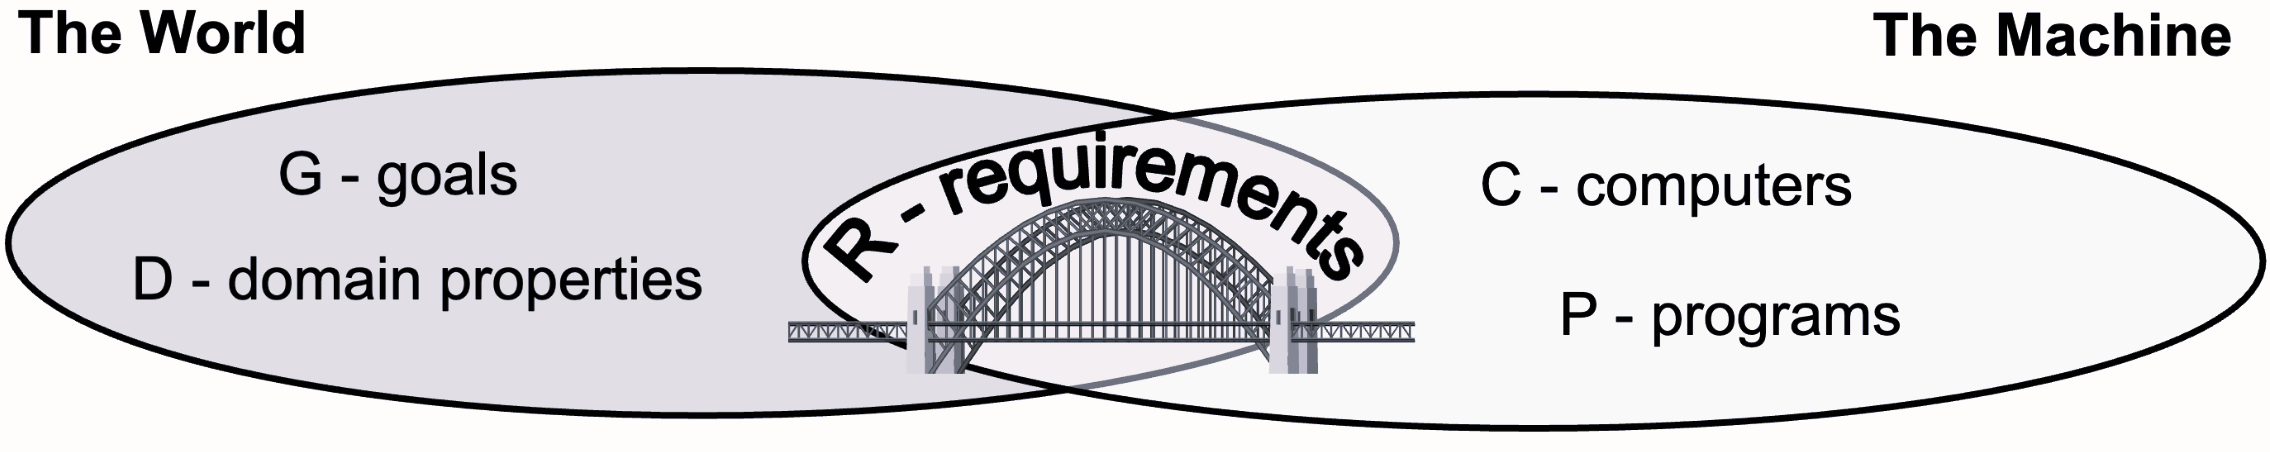
\includegraphics[width=0.75\linewidth]{images/worldmachine.png}
        \caption{Goals, domain assumptions, and requirements}
    \end{figure}
    Goals are prescriptive assertions formulated in terms of world phenomena (not necessarily shared). Domains properties/assumptions are descriptive assertions assumed to hold in 
    the world. Requirements are prescriptive assertions formulated in terms of shared phenomena. 
      
    The requirements $R$ are complete if: 
    \begin{itemize}
        \item $R$ ensures satisfaction of the goals $G$ in the context of the domain properties $D$, this means that $R\land D \models G$.
        \item $G$ adequately capture all the stakeholders' needs.
        \item $D$ represent valid properties/assumptions about the world.
    \end{itemize}

    \section{Elicitation of requirements}
    The complexity in requirement engineering can be coped with:
    \begin{itemize}
        \item Adopting different approaches and strategies and combining the results reached with all of them.
        \item Being as close as possible to stakeholders.
        \item Letting stakeholders describing their viewpoints.
    \end{itemize}
    The scenario can be generalized in term of:
    \begin{itemize}
        \item Participation actors.
        \item Describe the entry condition.
        \item Describe the flow of events.
        \item Describe the exit condition.
        \item Describe exceptions.
        \item Describe special requirements.
    \end{itemize}

    \section{Modeling requirements}
    \begin{definition}
        A \emph{model} is a representation in a certain medium of something in the same or another medium. The model captures the important aspects of the thing being modeled and 
        simplifies or omits the rest. 
    \end{definition}
    The reality $R$ is composed by: real things, people, processes and relationship. The model $M$ is an abstraction of things, people, processes and relationship between these 
    abstraction. 
     
    The reality needs to be interpreted ($I$) with a mapping function. To have a good model the relationships that are valid in the reality $R$ need to be valid also in the 
    model $M$.
    \begin{figure}[H]
        \centering
        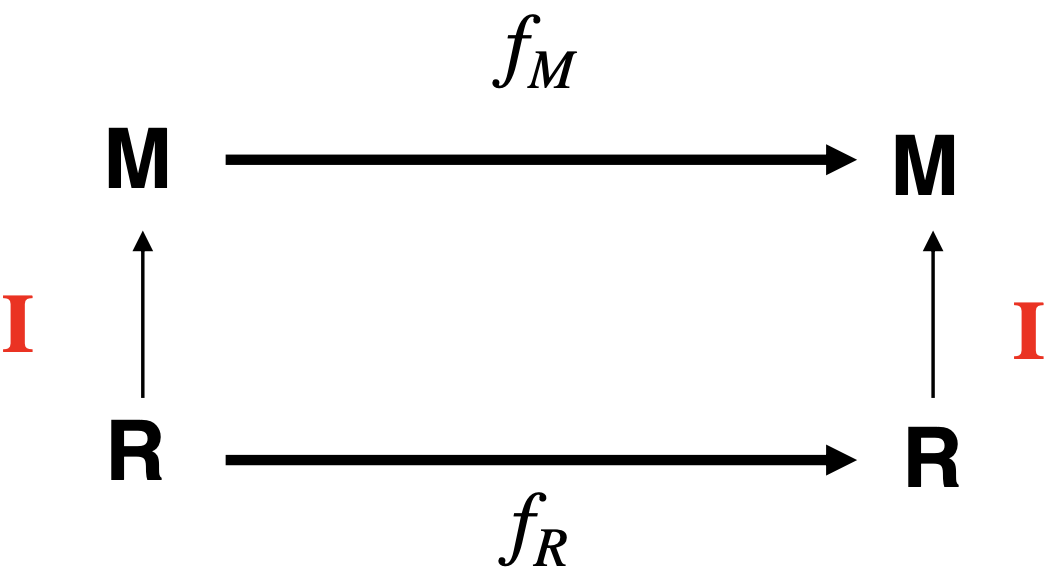
\includegraphics[width=0.5\linewidth]{images/modeling.png}
        \caption{Relationship between model $M$ and reality $R$}
    \end{figure}
    The software models are used for: 
    \begin{itemize}
        \item Capture and precisely state requirements and domain knowledge.
        \item Think about the design of a software system Generate usable work products.
        \item Give a simplified view of complex systems Evaluate and simulate a complex system.
        \item Generate potential configurations of systems.
    \end{itemize}
    The principal modeling issues are coherence (different views of the system must be coherent) and variation in interpretation and ambiguity (define where different 
    interpretation of the model are acceptable).
     
    In requirements engineering we should only model:
    \begin{itemize}
        \item The objects and people that are of interest for the given problem.
        \item The relevant phenomena.
        \item The goals, requirements, and domain assumptions.
    \end{itemize}
    The tool that we can use for modeling are: 
    \begin{itemize}
        \item Natural language (English, Italian, $\dots$):
        \begin{itemize}
            \item Pros: simplicity of use.
            \item Cons: high level of ambiguity, it is easy to forget to include relevant information.
        \end{itemize}
        \item Formal language (FOL, Alloy, Z, $\dots$):
        \begin{itemize}
            \item Pros: possibility to use tool to support analysis and validation, the approach forces the user in specifying all relevant details.
            \item Cons: you need to be expert in the use of the language.
        \end{itemize}
        \item Semi-formal language (UML):
        \begin{itemize}
            \item Pros: simpler than a formal language, impose some kind of structure in the models.
            \item Cons: not amenable for automated analysis, some level of ambiguity.
        \end{itemize}
        \item Mixed approach: use a semi-formal language for the basics. Comment and complement the semi-formal models with explanatory informal text. use a formal language for the 
        most critical parts.
    \end{itemize}

    \section{Use cases and requirements}
    The main steps when formulating use cases are: 
    \begin{enumerate}
        \item Name the use case
        \item Find the actors: generalize the concrete names to participating actors.
        \item Concentrate on the flows of events, entry and exit condition using natural language.
        \item Focus on exceptional cases and special requirements.
    \end{enumerate}
    Each use case may lead to one or more requirements.
     
    A use case is a flow of events in the system, including interaction with actors. The use cases are initialized by an actor and has a termination condition. 
    \begin{definition}
        The \emph{use case model} is the set of all use cases specifying the complete functionality of the system. 
    \end{definition}
    \begin{definition}
        A \emph{use case association} is a relationship between use cases. The principal types of use case association are: 
        \begin{itemize}
            \item Include(a use case uses another use case).
            \item Extends (a use case extends another use case).
            \item Generalization (an abstract use case has several different specializations).
        \end{itemize}
    \end{definition}
    \begin{figure}[H]
        \centering
        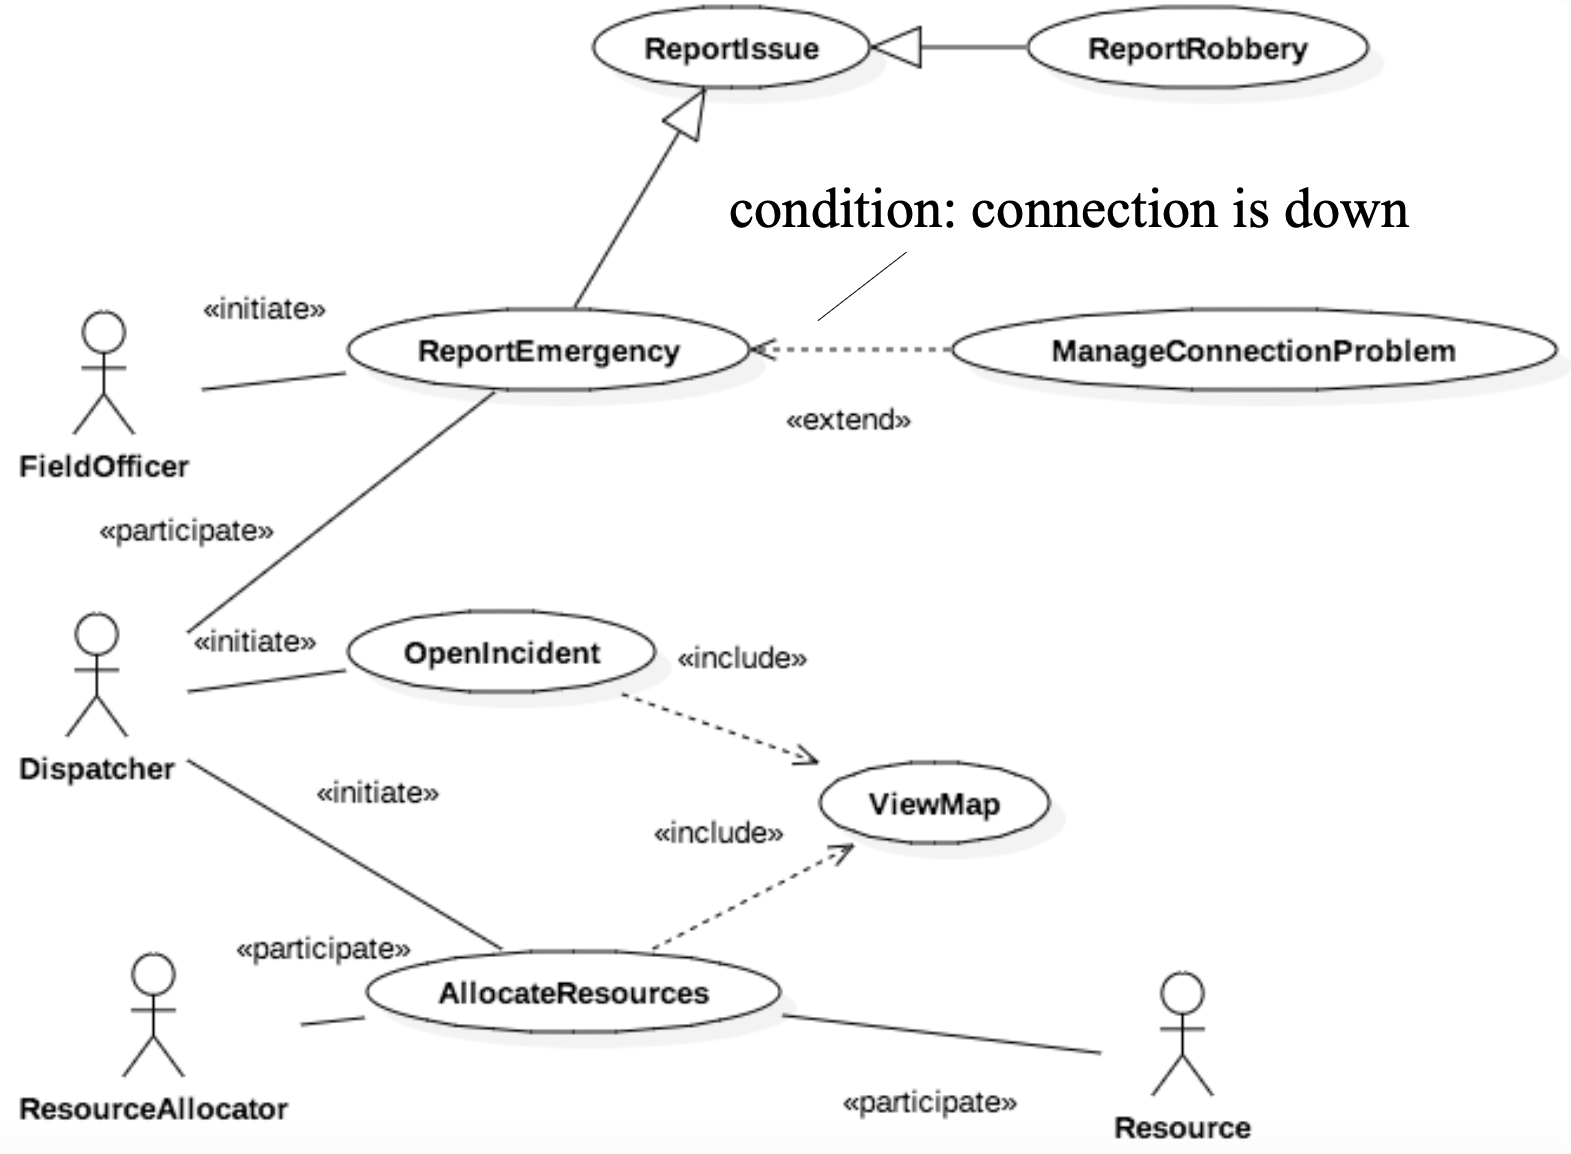
\includegraphics[width=0.5\linewidth]{images/usecase.png}
        \caption{Use case model example}
    \end{figure}
\section{Requirements-level class diagrams}
    The requirements-level class diagrams are conceptual models for the application domain. They may model objects that will not be represented in the software-to-be. Usually, the 
    do not attach operations to objects: it's best to postpone this kind of decisions until software design. 
     
    To find objects and classes we need to:
    \begin{itemize}
        \item Analyze any description of the problem and application domain you may have.
        \item Analyze your scenarios and use cases descriptions.
    \end{itemize}
    Finding objects is the central piece in object modeling. A possible tool to use in the analysis is the Abbott Textual Analysis also called noun-verb analysis: nouns are good 
    candidates for classes and verbs are good candidates for associations and operations. 
    \begin{figure}[H]
        \centering
        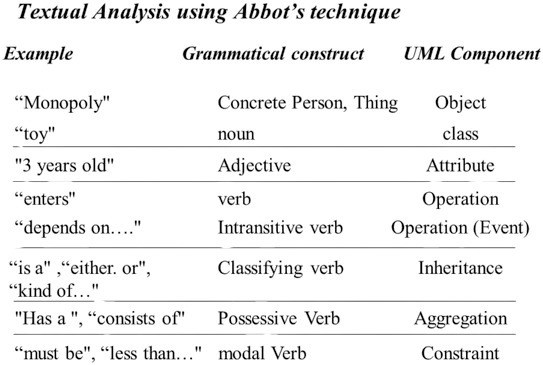
\includegraphics[width=0.5\linewidth]{images/Abbott.png}
        \caption{Abbott Textual Analysis example}
    \end{figure}
\section{Dynamic modeling}
    The purpose of the dynamic modeling is to supply methods to model interactions, behaviours of participants and workflow. This can be done with: sequence diagram, state machine 
    diagram and activity diagram. Some objects can be found whilst completing those diagrams.
     
    The sequence diagram is created following the flow of events in the use case diagram. A sequence diagram is a graphical description of objects participating in a use case 
    scenario using a Directed Acyclic Graph notation.
    The principal rules to create a sequence diagrams are: 
    \begin{itemize}
        \item An event always has a sender and a receiver.
        \item The representation of the event is sometimes called a message.
        \item Find sender and receiver for each event.
    \end{itemize}
    \begin{figure}[H]
        \centering
        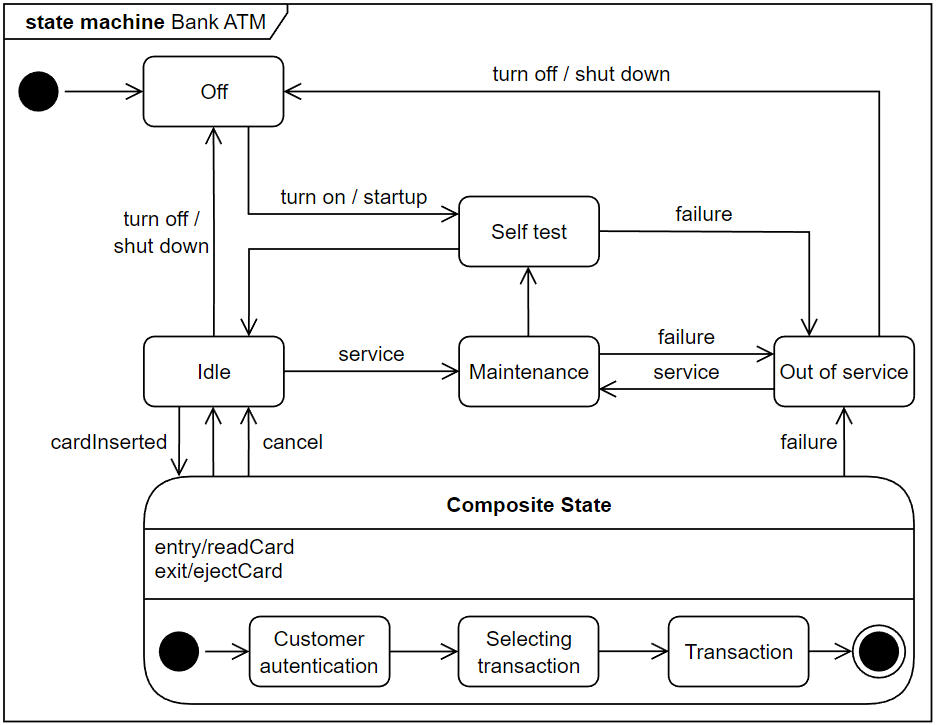
\includegraphics[width=0.5\linewidth]{images/state.png}
        \caption{Example of a state diagram}
    \end{figure}
     
    For a good dynamic modeling we ha to construct a model only for classes with significant dynamic behaviour and consider only relevant attributes. We have also to look ate the
    granularity of the application when deciding on actions and activities and reduce notational clutter.

\newpage

\chapter{Alloy}
    \section{Definition}
        Alloy is a formal notation for specifying models of systems and software. It looks like a declarative object oriented language, but also has a mathematical foundation.
         
        Alloy comes with a supporting tool to simulate specifications and performs property verification.
         
        Alloy has been created to offer an expressive power similar to the Z language as well as the strong automated analysis of the SMW model checker. 
         
        Alloy can be used in requirement engineering  to formally describe the domain and its properties, or operations that the machine has to provide. In software design Alloy can be used to formally model components and their interactions. 
    \section{Introduction}
        Alloy is a mixture of first order logic and relational calculus. The main elements of this formal language are: 
        \begin{itemize}
            \item Carefully chosen subset of relational algebra (uniform model for individuals, sets and relations; no high-order relations).
            \item Almost no arithmetic.
            \item Modules and hierarchies.
            \item Suitable for small, explanatory specification.
            \item Powerful and fast analysis tool.
        \end{itemize}
    \section{Syntax}
        Alloy shows bounded snapshots of the world that satisfy the specification. Allow does bounded exhaustive search for counterexample to a claimed property using SAT.
        \begin{definition}
            \emph{Atoms} are Alloy's primitive entities (indivisible, immutable and uninterpreted). 
        \end{definition}
        \begin{definition}
            \emph{Relations} associate atoms with one another (set of tuples; tuples are sequence of atoms).
        \end{definition}
        The relations in Alloy are typed. The relation type is determined by the declaration of the relation. The basic Alloy relations type are: $none$ (empty set), $univ$ (universal set) and $iden$ (identity relation). The logic operators in Alloy are: 
        \begin{itemize}
            \item Union $\cup$.
            \item Intersection $\&$.
            \item Difference $-$.
            \item Subset $in$.
            \item Equality $=$.
            \item Cross product $\rightarrow$ (similar to a natural join). 
            \item Dot join $.$ or $[\:]$ (the last element of the first relation joins on the corresponding first elements of the second relation, and then removes the element from the relation).
        \end{itemize}
        The possible binary closures on the relations are: 
        \begin{itemize}
            \item Transpose $\sim$ (inverts the order of the elements in the relation).
            \item Transitive $\land$ ($^{\land}r=r+r.r+r.r.r+\dots$). 
            \item Reflexive transitive $*$ ($^{*}r=iden+^{\land}r$)
        \end{itemize}
        The possible restrictions are: 
        \begin{itemize}
            \item Domain restriction $<:$, that restricts the elements on the left side to the set on the right side.
            \item Range restriction $:>$, that is same as before but the relations are inverted. 
            \item Override $++$, that removes the tuples on the left that are in the right relations and adds all the remaining relations of the right relation. 
        \end{itemize}
        The Alloy Boolean operators are the following: negation ($!$ or $not$), conjunction ($\&$ or $and$), disjunction ($\mid \mid$ or $or$), implication ($\implies$ or $implies$), alternative ($,$ or $else$) and bi-implication ($\iff$ or $iff$). The alloy logic quantifiers are: 
        \begin{itemize}
            \item $all$: holds for every element.
            \item $some$: holds for at least one element.
            \item $no$: holds for no elements.
            \item $lone$: holds for at most one element.
            \item $one$: holds for exactly one element.
        \end{itemize}
        To define a relation with a singleton we can use the following declaration: 
        \[x \: : \: m \: e\]
        Where $x$ is the name of the relation, $m$ is the multiplicity of the element (that can be: $set$, $one$, $lone$ or $some$) and $e$ is the name of the element in the relation. If the relation is composed by couple the declaration became like this: 
        \[r \: : \: A \: m \: \rightarrow \: n \: B\]
        Where $r$ is the name of the relation, $A$ and $B$ are the name of the elements with multiplicity $m$ and $n$ respectively.
         
        $let$ is used to define a formula or expression that can be reused. Other useful operators are: $\# r$ (that define the number of tuples in $r$), $0,1,\dots$ (integer used to define the value of some variables or constants), $+$ (plus), $-$ (minus), all the comparison operators ($<$, $<=$, $=$, $=>$, $>$). There is also the operator $sum$ that adds all the elements in the selected tuple. 

        \section{Address book example}
        Imagine that we are asked to model a very simple address book. The books that contain a bunch of addresses linked to the corresponding names. 
        
        In this example we have three entities, which are: $Name$, $Addr$ and $Book$.
        $addr$ is linking $Name$ to $Addr$ within the context of $Book$. To indicate this relation we use the keyword $lone$ that indicates that each $Name$ can correspond at most one 
        $Addr$. We can resume the previous statements as:
        \begin{algorithmic}[H]
            \State \textbf{sig} Name $\{\}$
            \State \textbf{sig} Addr $\{\}$
            \State \textbf{sig} Book $\{$ 
            \State \:\:\:\:\:\: addr: Name -$>$ \textbf{lone} Addr 
            \State $\}$
        \end{algorithmic}
        This specification creates the following relations: 
        \begin{itemize}
            \item Sets are unary relations.
            \item Scalars are singleton sets.
            \item The ternary relation involving the three predicates.
        \end{itemize}
        We can declare a new predicate with the keyword $pred$. 
        \begin{algorithmic}[H]
            \State \textbf{pred} show $\{\}$
            \State \textbf{run} show \textbf{for} 3 \textbf{but exactly} 1 Book
        \end{algorithmic}
        Where the second line indicates that we need to find at most three elements for every $Book$. The predicate $show$ defined previously is empty and return always $true$. Now we 
        can define a predicate with some argument, for example: 
        \newpage
        \begin{algorithmic}[h]
            \State \textbf{pred} show [b:Book]$\{$
            \State \:\:\:\:\:\: $\#$ b.addr $>$ 1
            \State $\}$
            \State \textbf{run} show \textbf{for} 3 \textbf{but exactly} 1 Book
        \end{algorithmic} 
        The predicate (consistent) in the previous example adds a constraint on the number of $Address$ relations in a given $Book$. 
        The predicate (consistent) in the following example adds a constraint on the number of different $Address$ that appears in the $Book$.
        \begin{algorithmic}[H]
            \State \textbf{pred} show [b:Book]$\{$
            \State \:\:\:\:\:\: $\#$ b.addr $>$ 1
            \State \:\:\:\:\:\: $\#$ Name.(b.addr) $>$ 1
            \State $\}$
            \State \textbf{run} show \textbf{for} 3 \textbf{but exactly} 1 Book
        \end{algorithmic}
        The predicate (inconsistent) in the following example contains the keyword $some$ that indicates the existence of an element. In this case we have only one $Book$ so the tool 
        will say that no instances can be found. 
        \begin{algorithmic}[H]
            \State \textbf{pred} add [b:Book]$\{$
            \State \:\:\:\:\:\: $\#$ b.addr $>$ 1
            \State \:\:\:\:\:\: \textbf{some} n:Name $\mid$ $\#$ n.(b.addr) $>$ 1
            \State $\}$
            \State \textbf{run} show \textbf{for} 3 \textbf{but exactly} 1 Book
        \end{algorithmic} 
        All the previous predicates are static because they doesn't change the signature. In Alloy there are also dynamic predicates for dynamic analysis. For example we can define a 
        predicate that adds an $Address$ and $Name$ to a $Book$ in the following way: 
        \begin{algorithmic}[H]
            \State \textbf{pred} add [b,b':Book, n:Name,a:Addr]$\{$
            \State \:\:\:\:\:\:\:\: b'.addr=b.addr + n -$>$ a
            \State $\}$
            \State \textbf{pred} showAdd [b,b':Book, n:Name,a:Addr]$\{$
            \State \:\:\:\:\:\:\:\: add[b,b',n,a]
            \State \:\:\:\:\:\:\:\: $\#$Name.(b'.addr) $>$ 1
            \State $\}$
            \State \textbf{run} showAdd
        \end{algorithmic} 
        We can now define a predicate for the $Book$ deletions.  
        \begin{algorithmic}[H]
            \State \textbf{pred} del [b,b':Book, n:Name]$\{$
            \State \:\:\:\:\:\:\:\: b'.addr=b.addr - n -$>$ Addr
            \State $\}$
        \end{algorithmic} 
        We can check if running a delete after an add returns us in the initial situation or not by using an $assertion$:
        \begin{algorithmic}[H]
            \State \textbf{assert} delRevertsAdd$\{$
            \State \:\:\:\:\:\:\:\: \textbf{all} b1,b2,b3:Book,n:Name,a:Addr
            \State \:\:\:\:\:\:\:\: add[b1,b2,n,a] \textbf{and} del[b2,b3,n] 
            \State \:\:\:\:\:\:\:\: \textbf{implies} b1.addr=b3.addr
            \State $\}$
        \end{algorithmic} 
        While checking an assertion, Alloy searches for counterexamples. In this case we will find a counterexample so the assert will result $false$. To correct the assert we need to 
        modify it in the following way: 
        \begin{algorithmic}[H]
            \State \textbf{assert} delUndoesAdd$\{$
            \State \:\:\:\:\:\:\:\: \textbf{all} b1,b2,b3:Book,n:Name,a:Addr $\mid$
            \State \:\:\:\:\:\:\:\: \textbf{no} n.(b1.addr) \textbf{and} add[b1,b2,n,a] \textbf{and} del[b1,b2,n]
            \State \:\:\:\:\:\:\:\: \textbf{implies} b1.addr=b3.addr
            \State $\}$
        \end{algorithmic} 
        We can also need to get some signature. To do that we can use the Alloy functions. For example we can declare a function that search a certain $Book$ and return a set of $Address$:
        \begin{algorithmic}[H]
            \State \textbf{fun} lookup[b:Book,n:Name]: \textbf{set} Addr$\{$
            \State \:\:\:\:\:\:\:\: n.(n.addr)
            \State $\}$
        \end{algorithmic} 
    
        \section{Family relations example}
        We now consider a family relationship tree. First of all we have to define a generic person, that can be a men or a woman.
        \begin{algorithmic}[H]
            \State \textbf{abstract sig} Person $\{$
            \State \:\:\:\:\:\:\:\: father: \textbf{lone} Man 
            \State \:\:\:\:\:\:\:\: mother: \textbf{lone} Woman
            \State $\}$
            \State \textbf{sig} Man \textbf{extends} Person $\{$
            \State \:\:\:\:\:\:\:\: wife: \textbf{lone} Woman 
            \State $\}$
            \State \textbf{sig} Woman \textbf{extends} Person $\{$
            \State \:\:\:\:\:\:\:\: husband: \textbf{lone} Man 
            \State $\}$
        \end{algorithmic} 
        We have set that each $Person$ has at most one father and one mother (keyword $lone$) because we need a root for the tree. The person at the root needs to have no parents 
        (for example they are unknown). The signature $Person$ is $abstract$ because it needs to be specialized in one of the subsequent signatures, that are $Man$ or $Woman$.
        Signatures by using keyword $sig$ represents a set of atoms. Before this keyword we can define the number of entities that we need ($lone$, $one$ or $some$).
        \begin{definition}
            The \emph{fields} of a signature are relations whose domain is a subset of the signature. The keyword \emph{extends} is used to declare a subset of signature. 
        \end{definition}
        To get the set of grandpas of a given person we can define a function like this: 
        \begin{algorithmic}[H]
            \State \textbf{fun} grandpas[p:Person]:set Person $\{$
            \State \:\:\:\:\:\:\:\: p.(mother+father).father
            \State $\}$
            \State \textbf{pred} ownGrandpa[p:Person] $\{$
            \State \:\:\:\:\:\:\:\: p \textbf{in} p.grandpas[p]
            \State $\}$
        \end{algorithmic} 
        We have also defined a predicate that checks if the person is in the set of grandpas returned by the function $grandpas$. The problem now is that we have not set constraints 
        on relations. To do that we need to define two new operators for binary relations:
        \begin{itemize}
            \item Transitive closure: \textasciicircum $r=r+r.r+r.r.r+\dots$
            \item Reflex transitive closure: $*r=iden+$\textasciicircum$r$
        \end{itemize}
        We can now define that no one can be the father/mother of himself: 
        \begin{algorithmic}[H]
            \State \textbf{fact} $\{$
            \State \:\:\:\:\:\:\:\: \textbf{no} p:Person $\mid$ p \textbf{in} p.\textasciicircum(mother+father)
            \State $\}$
        \end{algorithmic} 
        We have also to set a constraint that if X is husband of Y, then Y is the wife of X:
        \begin{algorithmic}[H]
            \State \textbf{fact} $\{$
            \State \:\:\:\:\:\:\:\: \textbf{all} m:Man,w:Woman $\mid$ m.wife=w \textbf{iff} w.husband=m
            \State $\}$
            \State \textbf{fact} $\{$
            \State \:\:\:\:\:\:\:\: wife = \textasciitilde husband
            \State $\}$
        \end{algorithmic} 
        The two facts are equivalent, but the second has been written using the transpose operator. The fact can contains multiple constraints. So the previous constraints can be written 
        in one fact. The difference between $fact$ and $pred$ is that the first are global, while the second needs to be invoked.
    
    \newpage




    

    
\end{document}